\documentclass[11pt]{article}
\pdfoutput=1
\usepackage[margin=1in]{geometry}
\usepackage[T1]{fontenc}
\usepackage[utf8]{inputenc}
\usepackage{lmodern,microtype,booktabs,graphicx,amsmath}
\usepackage[numbers,sort&compress]{natbib}
\usepackage[hidelinks]{hyperref}
\usepackage{caption}
\captionsetup{font=small,labelfont=bf}
\hypersetup{pdftitle={Evaluating a Modular Mix-to-MIDI Pipeline on Slakh2100},
            pdfauthor={John Hurliman}}
\newcommand{\jams}{\texttt{jams}}
\newcommand{\ci}[2]{{\small[#1, #2]}}
\title{\textbf{Evaluating a Modular Mix-to-MIDI Pipeline\\on Slakh2100}}
\author{John Hurliman\\\small Independent researcher\\
\small \texttt{jhurliman@jhurliman.org}}
\date{September 2026}
\begin{document}
\maketitle

\begin{abstract}
In a modular audio-to-MIDI system, source separation and note transcription must be
evaluated together: improvement at an intermediate stage need not improve the final
output. We present a retrospective case study of \jams{}, an open-source pipeline,
using reported experiments on the Slakh2100-redux test split. For grouped non-bass
pitched accompaniment, replacing basic-pitch with YourMT3+ increases mean
onset-and-pitch F1 from 0.4733 to 0.7877 after the same SCNet separator. With reference
stems as input, the corresponding scores are 0.4897 and 0.8488. The larger transcriber
therefore retains an advantage despite separation errors in this configuration.
A second comparison finds opposite directions of change in drum SI-SDR and
downstream onset F1, without establishing a statistically reliable reversal.
These observations support measuring the complete cascade; they do not establish
that separation improves transcription, and do not measure performance on real electronic dance music.
We specify the scoring and aggregation conventions, commit the per-recording score
archives for the Slakh comparisons with checksums, and recompute every mean and
interval of those comparisons from them; the structure intervals in the appendix
are likewise recomputed from committed per-track predictions, while the secondary
key, tempo, and drum results remain reported values, and only one transcription
arm's note predictions were archived.
\end{abstract}

\section{Introduction}
An audio-to-MIDI application may use a separator to expose instrument groups, then
apply a different transcriber to each group. This arrangement offers editable stems
alongside symbolic output, but introduces two coupled sources of error. A separator
can remove useful note information or introduce interference that changes a
transcriber's predictions. Conversely, a stronger transcriber may recover more
notes from imperfect stems than a weaker transcriber recovers from reference audio.
The practical question is which component change improves the output a user receives.

We investigate this question through the mix-to-MIDI component of \jams{}, a local
music-analysis service.\footnote{This project is separate from the JAMS annotation
format and library at \url{https://github.com/marl/jams}.} The study uses existing pretrained models and previously
recorded Slakh2100 experiments. Its contribution is a specified component comparison
and an account of what that comparison supports, rather than a new neural
architecture. We distinguish three contrasts: changing the transcriber on reference
stems; changing it after a fixed separator; and changing the separator while holding
the transcriber fixed. The main analysis concerns grouped pitched accompaniment,
called \emph{other} by the separator. This is a polyphonic group, not an individual
instrument.

The first two contrasts give the clearest result: the reported YourMT3+ advantage
over basic-pitch persists after separation. The third is a diagnostic observation:
two separators have different orderings under drum SI-SDR and downstream onset F1.
Neither establishes that a cascade is better than direct mixture transcription,
which was not measured under the same protocol. Appendices retain secondary system
results and methodological qualifications.

\section{Related work and scope}
Separation followed by transcription is an established design; for example,
Derby et al.~\citep{derby2024pipeline} describe a modular route from mixtures to
stems, MIDI, and notation. Slakh2100~\citep{manilow2019slakh} supplies synthesized
multitracks and aligned MIDI suitable for examining both stages. Its grouped stems
allow a reference-input condition without assuming that reference input is an
upper bound on a transcriber's score.

Basic-pitch~\citep{bittner2022basicpitch} is designed for lightweight,
instrument-agnostic transcription. MT3~\citep{gardner2022mt3} and
YourMT3+~\citep{chang2024yourmt3} instead use sequence models for multi-instrument
transcription. YourMT3+ incorporates Slakh training data and stem augmentation;
our comparison does not control training data, model capacity, or computational
cost. Its original evaluation also addresses instrument identity and note offsets,
which our main metric omits. Recent lightweight models, including the Harmonica
preprint~\citep{ou2026harmonica}, further limit any interpretation of basic-pitch
as representative of the best current transcription systems.

We use HT-Demucs~\citep{rouard2023hybrid} and a released SCNet
variant~\citep{tong2024scnet} for the principal separator comparison. Their
architecture papers establish the methods, not the provenance or performance of
every subsequently released checkpoint. SI-SDR~\citep{leroux2019sdr} measures
waveform reconstruction, whereas note F1 measures agreement between discrete events.
There is no monotonic relationship implied by their definitions. This study
examines component selection within one pipeline, not a general ranking of model
families.

\section{System and evaluation protocol}
\label{sec:protocol}
\subsection{Pipeline and evaluated configurations}
The service accepts audio and returns separated audio files and per-group MIDI.
Separation produces drums, bass, other, and vocals. Pitched groups are transcribed
with basic-pitch or YourMT3+; a separate drum model produces percussion onsets.
The historical experiments analyzed here used an ADTOF-derived drum port
\citep{zehren2021adtof}. That port was subsequently replaced, so these measurements
describe the recorded configuration rather than every current service default.

For SCNet, the worker identifies the MSST release \texttt{v1.0.15}, configuration
\path{config_musdb18_scnet_xl_more_wide_v5.yaml}, and weights
\path{model_scnet_ep_36_sdr_10.0891.ckpt}. The repository calls this
configuration ``SCNet XL IHF.'' The pitched transformer is recorded as
YourMT3+ \texttt{YPTF.MoE+Multi}, invoked through \texttt{mt3-infer} and decoded
from 16\,kHz mono input. Basic-pitch uses its ICASSP 2022 checkpoint. For other,
the recorded onset/frame thresholds are 0.60/0.25, selected in a preliminary
babyslakh sweep; the worker also specifies a 58\,ms minimum note length.

Only the other group is central to the analysis because bass processing adds a
monophonic filter and a fixed octave transposition (Appendix~\ref{app:bass}).
Instrument labels are discarded within each pitched group. Beat-grid quantization
is disabled during evaluation. Model environments are separated into subprocesses,
but some dependency declarations are version ranges and external model downloads
lack cryptographic digests. This is useful execution isolation, not a guarantee
of bitwise reproduction.

\subsection{Dataset, grouping, and exclusions}
The experiment ledger identifies the Slakh2100-redux test split, with 151
multitracks. The acquisition script groups stems marked as drums into drums,
General MIDI bass programs 32--39 (zero-indexed), or stems labeled Bass, into bass,
and all remaining pitched stems into other. It sums audio within each group and
merges the corresponding MIDI instruments. An audit of all 445 grouped references
(151 multitracks; 8 have no bass stem) found no stem whose MIDI was merged while its
audio was unreadable, no truncation of a group to a shorter member, no clipping in
the 16-bit sums (largest summed peak 0.93), grouped audio equal to the recomputed
sums to one quantization step, and no note beyond the audio end. Cross-correlating
each group's onset-strength envelope with its MIDI onsets over $\pm$500\,ms puts
the global maximum between 0 and 70\,ms after note-on for 417 of the 445 groups
(class-wise 12--58\,ms, consistent with instrument attack times plus the
estimator's one-frame bias). The other 28 (22 drums, 3 bass, 3 other) have their
global peak elsewhere, at a one-beat multiple on periodic parts; for 20 of them the
near-zero peak is within 10\% of the global one and for 8 it is at 79--90\%.
Separately, six dense accompaniment groups have correlation below 0.3 throughout
(five of them with near-zero maxima), so the estimate is uninformative there. For
these groups the method cannot exclude an offset, though none shows a consistent
shift. The audit script and report are in the repository. Slakh contains synthesized instrumental
music; there is no reference vocal group in this evaluation.

The historical summary reports 151 accompaniment pairs and 143 bass pairs in the
reference-input comparison. A missing reference group is excluded from that
group's mean; an existing reference with no predicted notes scores zero. Failures
and missing groups must therefore be reported separately. The end-to-end archives
record 151 completed multitracks, zero pipeline failures, and 143 eligible bass
pairs, the same support as the reference-input comparison.

These are retrospective development results. The ledger records selection of
components after examining Slakh test performance. It does not establish an
untouched, confirmatory test of the complete pipeline. YourMT3+ was trained on
Slakh's training split according to its authors, so this is not zero-shot evaluation
on an unseen dataset. Exact checkpoint and split identities, including the
preliminary babyslakh development IDs, require archival verification. Source-MIDI
overlap across splits is a separate question from matching local filenames.

\subsection{Metrics and statistical interpretation}
For each multitrack and pitched group, reference and estimated notes are matched
one-to-one using \texttt{mir\_eval}~\citep{raffel2014mireval}, with 50\,ms onset
and 50-cent pitch tolerances and no offset criterion. Precision and recall are
computed from matched notes, with $F_1=2PR/(P+R)$. The corpus score is the arithmetic
mean of per-multitrack F1 over eligible reference groups, not F1 computed after
pooling all notes. Instrument identity, velocity, and notation quality are not
measured by this score.

For two systems A and B on the same eligible tracks, the paired effect is
\begin{equation}
 \widehat\Delta_{A-B}=\frac{1}{n}\sum_{i=1}^{n}(F_{1,i}^{A}-F_{1,i}^{B}).
\end{equation}
The archived reference-input analysis reports a percentile bootstrap with 10,000
track resamples and seed 0. Its intervals describe uncertainty conditional on these
trained models, track selection, and scoring choices. They do not account for
training-seed variation, prior test-set reuse, or dependence between arrangements
derived from related MIDI. We retain the reported intervals, identify them as
archival summaries, and make no multiplicity-adjusted confirmatory claims.

Drum onset F1 uses five classes: kick, snare, hi-hat, tom, and cymbal. The scorer
averages class F1 within a multitrack, including a class if either reference or
estimate contains it, then averages across multitracks. Absent reference classes
with false detections contribute zero. The SI-SDR implementation downmixes to mono,
resamples the estimate to the reference rate, and truncates to the shorter signal.
For reference $s$ and estimate $\hat s$, it computes
\begin{equation}
 \alpha=\frac{\langle\hat s,s\rangle}{\|s\|^2},\qquad
 \mathrm{SI\text{-}SDR}=10\log_{10}
 \frac{\|\alpha s\|^2}{\|\hat s-\alpha s\|^2},
\end{equation}
with $10^{-9}$ numerical stabilizers, no explicit mean removal or time-alignment
search, and subsequent averaging in dB. Silent reference signals are excluded.
These details distinguish the implementation from other SDR protocols.

\section{Results}
\subsection{Changing the transcriber}
\begin{table}[t]
\centering\small
\caption{Reported accompaniment (other) onset-and-pitch F1 on Slakh2100-redux,
$n=151$. Reference input is the summed ground-truth group. Brackets are 95\%
percentile bootstrap intervals (10,000 track resamples, seed 0) recomputed from the
committed per-track score archives. T1/T2b/S4/T10 identify runs in the project ledger.}
\label{tab:transcription}
\begin{tabular}{llll}
\toprule
Input & Transcriber & Mean F1 [95\% CI] & Run \\
\midrule
Reference other & basic-pitch & 0.4897 [0.4742, 0.5055] & T1 \\
Reference other & YourMT3+ & 0.8488 [0.8369, 0.8607] & T2b \\
SCNet other & basic-pitch & 0.4733 & S4 \\
SCNet other & YourMT3+ & 0.7877 & T10 \\
\bottomrule
\end{tabular}

\end{table}
\begin{figure}[t]
\centering
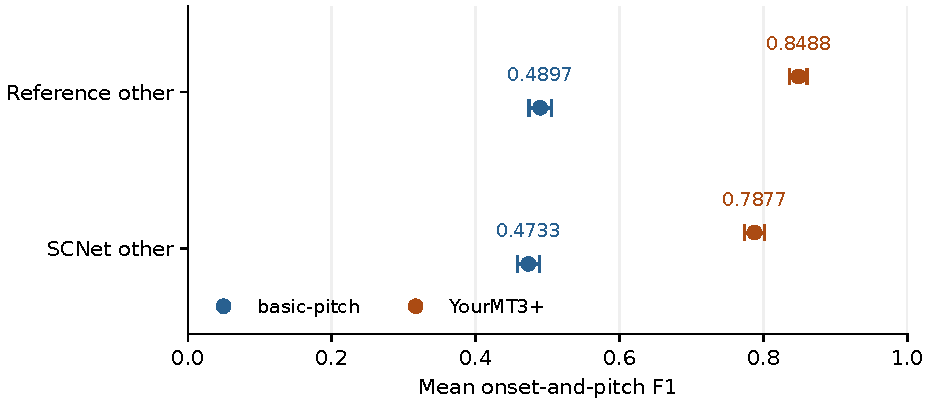
\includegraphics[width=0.82\linewidth]{figs/fig_transcription.pdf}
\caption{The transcriber comparison under two input conditions
(Table~\ref{tab:transcription}). Separation is fixed for the mix-input condition.
Intervals are recomputed from the committed per-track score archives; no
predictions were regenerated.}
\label{fig:transcription}
\end{figure}

With reference accompaniment as input, the recorded mean F1 is 0.4897 for
basic-pitch and 0.8488 for YourMT3+ (Table~\ref{tab:transcription}). The archived
paired difference is $+0.3591$ \ci{+0.3471}{+0.3713}, with YourMT3+ ahead on all
151 pairs. This is the strongest numerical contrast in the study; recomputation
from the committed per-track archive reproduces the archived mean and interval
exactly.

After the same SCNet separator, the scores are 0.4733 and 0.7877, a paired
difference of $+0.3144$ \ci{+0.3017}{+0.3271}, again with YourMT3+ ahead on all
151 pairs. Relative to each model's reference-input score, separation is associated
with a decrease of $0.0164$ \ci{0.0136}{0.0193} for basic-pitch (lower on 135 of
151 tracks) and $0.0611$ \ci{0.0547}{0.0677} for YourMT3+ (lower on 149). The
larger absolute decrease for YourMT3+ does not reverse the model ordering. These
intervals are recomputed from the stored per-track scores; they inherit every
caveat of the original runs.

YourMT3+ after separation also exceeds basic-pitch on reference stems by 0.2980.
This compares two complete configurations with different transcribers, not a
violation of an ``oracle ceiling.'' A reference-input score is an observed
operating point, not a mathematical upper bound. The comparison supports upgrading
the transcriber in this particular pipeline. It does not show that improving
transcription is generally more valuable than improving separation, nor that the
gain comes from architecture alone.

\subsection{Changing the separator}
\begin{table}[t]
\centering\small
\caption{Reported separator comparison with basic-pitch for pitched groups and
the historical ADTOF port for drums, on the same 151-track test split (143
eligible bass pairs in both archives). Paired differences recomputed from the
per-track archives, SCNet minus HT-Demucs: other $+0.0148$ \ci{+0.0119}{+0.0176},
bass $+0.0490$ \ci{+0.0330}{+0.0656}, drums $-0.0104$ \ci{-0.0209}{+0.0004}.}
\label{tab:separation}
\begin{tabular}{lrrrrrr}
\toprule
 & \multicolumn{3}{c}{SI-SDR (dB)} & \multicolumn{3}{c}{Downstream F1} \\
\cmidrule(lr){2-4}\cmidrule(lr){5-7}
Separator & Drums & Bass & Other & Drums & Bass & Other \\
\midrule
HT-Demucs & 11.61 & 4.57 & 10.13 & 0.5845 & 0.5957 & 0.4585 \\
SCNet & 14.31 & 5.98 & 11.77 & 0.5741 & 0.6448 & 0.4733 \\
\bottomrule
\end{tabular}

\end{table}
SCNet has higher reported mean SI-SDR than HT-Demucs for all three groups
(Table~\ref{tab:separation}). Its downstream F1 is also higher for other and bass.
On drums, however, SI-SDR increases from 11.61 to 14.31\,dB while onset F1 decreases
from 0.5845 to 0.5741. The paired drum difference recomputed from the two archives
is $-0.0104$ \ci{-0.0209}{+0.0004}, with SCNet lower on 87 of 151 tracks and
higher on 63; the interval includes zero. The opposite directions in these averages
are therefore an observed discrepancy, not a demonstrated population-level reversal.

Differences in transient preservation are one possible explanation, but this
experiment does not isolate them. Decoder thresholds, interference, temporal
alignment, and the drum model's training distribution could also matter. The
limited operational implication is to measure transcription on separator output
instead of assuming an SI-SDR improvement will transfer to note accuracy.
Subset-only runs of other separators are retained in Appendix~\ref{app:subsets};
they are not ranked against full-split averages.

\section{Limitations and next evaluation}
The principal limitations affect interpretation, not just generality. First, the
component choices were informed by this test set. A fresh corpus with a frozen
configuration is needed for confirmatory evaluation. Second, the baseline comparison
jointly changes model capacity, training data, and inference cost. We did not measure
a quality--latency frontier. Third, an instrument-agnostic onset metric does not
establish usable note durations, instrument assignments, velocities, or editing effort.

The most informative missing control is \emph{the same YourMT3+ checkpoint on
the unseparated mixture}, scored against the same grouped references with an
explicit instrument-to-group mapping. Without that control, the incremental value
of separation is unknown. A new lightweight baseline should also be tested before
making claims about current model families. These comparisons should use a fixed
development split, record every failure, and archive per-track predictions and
resource use. They are proposed experiments, not previously completed work.

Slakh uses sample-rendered audio. The findings do not establish performance on real
EDM, recorded acoustic ensembles, or vocals. A real-audio evaluation and an editing
study would address those distinct questions. The bass transposition requires its
own audio/MIDI audit and sensitivity analysis before its scores can support a
general pitch-accuracy claim (Appendix~\ref{app:bass}).

\section{Conclusion}
The reported Slakh2100 experiments favor YourMT3+ over basic-pitch for grouped
accompaniment both with reference stems and after a fixed SCNet separator. They
also show that average waveform and downstream event metrics can move in opposite
directions. These are bounded observations about evaluated configurations. They
motivate paired evaluation of the complete pipeline, with explicit grouping,
scoring, and model provenance, while leaving the benefit of separation over direct
transcription unresolved.

\section*{Code and data availability}
Source code, the experiment ledger, and the evidence behind every number in this
paper are in the repository at \url{https://github.com/jhurliman/jams}. The five
per-recording score archives (runs T1, T2b, S4, T10, and the HT-Demucs run S1) and
the S4 SI-SDR aggregate are committed under \path{paper/evidence/} with SHA-256
checksums, and \path{paper/verify_results.py} recomputes every mean and paired
interval of the Slakh comparisons in Sections~3--4 from them (accompaniment rows,
the bass reference, and the separator table and deltas), refusing missing
archives, duplicate rows, or mismatched track sets. The raw gate predictions of
the structure experiments (all challenger and stock arms) are committed as well,
and \path{eval/structure_class_cis.py} recomputes every per-class and aggregate
interval of Appendix~C from them with complete held-out coverage, cross-checking
the archived scored artifacts per track. The key, tempo, and drum intervals in
the appendices are reported from the ledger and are not covered by this
recomputation. The tables and figure regenerate from a summary snapshot that records that
verification. The repository is the only hosting dependency; no cloud object store
is required to reproduce the analysis.

The YourMT3+ reference-input predictions (run T2b) were also saved. Rescoring
them from the raw note lists against independently rebuilt grouped Slakh
references, with the same scorer and library versions, reproduces every archived
per-track precision, recall, and F1 value exactly for all 151 accompaniment and 143
bass pairs (\path{paper/rescore_t2b.py}). The basic-pitch and end-to-end note
predictions were not saved, so those arms are verified at the stored-score level
only. Checkpoint identities, library versions, decoding parameters, and the items
that remain unrecoverable are recorded in \path{paper/PROVENANCE.md}. No model
inference was rerun for this revision, and no missing measurement has been
estimated or synthesized.

\section*{Acknowledgments and AI use}
We thank the authors and maintainers of the datasets, models, and evaluation
software cited in this paper. The original manuscript was generated with Claude
(Anthropic), which also assisted implementation and experiment execution under the
author's direction. OpenAI Codex assisted source checking, evaluation-code auditing,
and substantive manuscript revision. This use extends beyond language editing.
The named human author is responsible for the submitted work; neither system is
an author. The limits of the verification performed are stated above.

\appendix
\section{Bass and smaller separator experiments}
\label{app:bass}
The reference-input bass comparison has 143 eligible pairs in the archived
statistics, with F1 0.7889 for basic-pitch and 0.8486 for YourMT3+; the reported
paired difference is $+0.0597$ \ci{+0.0034}{+0.1100}. The YourMT3+ score follows
a fixed $+12$-semitone shift of the estimated bass notes and no other
post-processing: rescoring the archived predictions reproduces 0.8486 only with the
shift alone, whereas adding the service's monophonic filter would give 0.8126. The
service applies the shift in its orchestrator; the evaluation CLI also offers an
additional shift, so the exact arguments matter and are now documented.
The earlier manuscript called this a universal written-MIDI convention. The
repository's empirical observation on a small preview subset does not establish
that assertion. A renderer- and instrument-specific pitch audit, with shifted and
unshifted sensitivity results, is required. Bass is therefore excluded from the
main transcription claim.

\subsection{Subset-only separator runs}
\label{app:subsets}
HT-Demucs-ft was evaluated on 50 tracks and BS-RoFormer on 47. The ledger
attributes the latter restriction to an output-naming mismatch that left 104
tracks unmatched. Those missing outputs may be systematically different. Although
the ledger asserts a comparison to SCNet on the matched subset, that paired
result is not publicly reconstructible from the aggregate table. We retain these
runs in the ledger and make no cross-subset ranking here. Similarly, the earlier
loss from discarding guitar and piano outputs of a six-stem model is an integration
error, not evidence against that separation architecture.

\section{Key detection: corrected interpretation}
\label{app:key}
The project's K10 model is a small convolutional key classifier trained on
\texttt{beatport\_key}; its log-CQT input and absolute-frequency readout are
specified in \texttt{eval/train\_key\_cnn.py}. It is related to the convolutional
family of Korzeniowski and Widmer~\citep{korzeniowski2018genre}. The ledger reports
1,363 usable training examples and zero track-ID overlap with GiantSteps Key.
This check does not rule out duplicate recordings or prior use of the benchmark
for development. K10's motivation explicitly cites earlier GiantSteps test-error
analysis, and an older classifier was trained on that test set. A final model
being evaluated once does not make the entire development history blind to the
benchmark.

The historical summaries report K10 exact accuracy 0.7795 on 567 examples and
weighted score 0.8321, versus 0.7725 and 0.8328 for madmom's default processor.
The score implementation awards 0.5 for a same-mode fifth in \emph{either}
direction. This agrees with the definition in the 2018 paper but differs from
\texttt{mir\_eval} 0.8.2's ascending-fifth-only implementation. These scores must
retain that convention label. The official 2026 task implementation must be
checked before claiming protocol compatibility.

The archived paired weighted difference, $-0.0007$ \ci{-0.0187}{+0.0182},
does not establish superiority, equivalence, or non-inferiority. Equivalence would
require a justified margin and a corresponding analysis. These intervals are also
conditional on an already observed benchmark.

\subsection{Why the earlier subset explanation is invalid}
The previous draft attributed the difference between a published score of 0.746
and a local score of 0.8328 entirely to retaining 567 of 604 tracks. For nonnegative
scores and unchanged predictions, scoring, and labels, a subset mean obeys
\begin{equation}
 \overline s_{\rm subset}\leq \frac{N}{n}\overline s_{\rm full}.
\end{equation}
Even assigning zero to all excluded tracks gives
$604(0.746)/567=0.7947$, below 0.8328. Track exclusion alone cannot explain the
reported difference under the draft's own assumptions. Moreover, the 2018 article
reports a selected single model, whereas madmom's documented default processor
uses an ensemble. Checkpoint and annotation differences are further possibilities.
No causal attribution of the discrepancy is supported, and the earlier ``six times
the field's progress'' claim is withdrawn.

\section{Secondary tempo, drum, and structure results}
The ledger records a replacement tempo CNN and a replacement drum CRNN, separate
from the historical transcription experiments. The tempo comparison reports a
paired Acc1 difference of $-0.002$ \ci{-0.015}{+0.011} on 458 corrected-label
examples. The genre-informed octave resolver and label corrections are part of
that protocol, not intrinsic properties of the CNN. For drums, the reported
reference-stem macro onset F1 is 0.767 versus 0.638 on Slakh and 0.818 versus
0.645 on a 500-example E-GMD subset. These are not end-to-end results for the
replacement drum model. Partitions, aggregation, and archived outputs must be
recovered before further inferential claims; the acoustic-kit experiments in the
ledger also show weaker transfer than the synthetic results alone would suggest.

The structure experiments use the Raveform authors' released models
\citep{kim2026raveform}, with three locally trained challengers. The ledger records
failure of the stated acceptance criteria for reweighted training from scratch,
a frozen-trunk readout, and a residual readout. For the frozen readout on fold 2,
the reported cooldown-coverage gain is $+0.233$ \ci{+0.157}{+0.312}, while buildup
loses $0.158$ \ci{0.098}{0.219}; the residual readout loses $0.240$
\ci{0.175}{0.308} on buildup. These intervals, and those of the from-scratch
arms on both folds, are recomputed from the committed raw predictions of every
arm (165 held-out tracks on fold~2, 162 on fold~1, no missing or failed tracks);
the archived scored artifacts match the recomputation track by track, and the
frozen-readout arms reproduce the stock beat and boundary scores exactly. The code
averages the fraction correctly labeled within each reference segment, then
averages within each track and across eligible tracks. This is not
corpus-duration-weighted accuracy or a precision measure; overprediction can raise
coverage.

These outcomes show that the evaluated interventions did not meet their goals.
They do not identify label quality as the limiting cause or exhaust possible
architectures, objectives, and optimization choices. Reuse of fold 2, single
training runs, and sparse class support limit inference. No assertion that a
negative result needs no replication is made.

\bibliographystyle{unsrtnat}
\bibliography{references}
\end{document}
